\documentclass[11pt]{article}
\usepackage{cafestyle}
\usepackage{float}
% Every table is produced by R and included with \input; this macro shrinks wide ones.
\newcommand{\rtable}[1]{\resizebox{\ifdim\width>\textwidth\textwidth\else\width\fi}{!}{\input{tables/#1}}}

\title{How Big Are Prague's Caf\'es?\\\large Café Size --- Data Analytics Semestral Project}
\author{Anthony George}
\date{November 2026}

\begin{document}
\maketitle

\begin{abstract}
This report asks how big Prague's cafés are and whether their size goes together with their ratings and prices. It uses 195 cafés visited in person by the class in autumn 2026. The typical café is small: the median café has 22 seats inside, and the mean of 28 seats does not differ detectably from 30. Cafés have about 17 more seats inside than outside, and Prague~5 has fewer outdoor seats than Prague~1. Small cafés (15 or fewer seats inside) are top-rated about twice as often as larger ones. Bigger cafés are slightly more expensive, but the link is weak, depends on a few very large cafés, and is not clearly different from zero once distance from the Orloj is taken into account. In this sample, size says more about a café's rating than about its prices.
\end{abstract}

% =====================================================================
\section{Introduction}
This report is the \emph{Café Size} chapter of the class story about the Prague café market.
Seats are the most physical measure of a café, and they shape what kind of place it is: a three-table espresso bar, a neighbourhood café with a terrace, or a large Old Town café house. I therefore start by describing size: whether the average café seats about 30 people inside (A1), whether cafés with outdoor seating also have bigger interiors (A2), how many more seats cafés have inside than outside (A3), and whether outdoor seating is concentrated in some districts (A4). I then ask whether size goes together with quality and price: whether small cafés are more often top-rated (A5), and whether bigger cafés charge more, measured by the Price Level (A6--A10). The price questions build from a simple correlation to regressions that add the distance from the Orloj, outdoor seating and finally a logistic model of the chance of being an above-median-price café.

% =====================================================================
\section{Data and cleaning}
The café data were collected in autumn 2026, with each student logging 20 cafés; the raw data contained 299 rows, yet 99 of them were completely empty. Because cafés always have names, I removed every row that had neither a name nor an address, which left me with 200 cafés. Some cafés had been visited by two students. I couldn't base this solely on the name because of chains, so I counted two rows as the same café if the café names were the same and their coordinates were within 100\,m of each other. There were 5 repeated cafés; I kept the first entry of each repeated café, as a rule to prevent choosing data I preferred. With the cafés that were repeated, the seat count was occasionally different. Along with that, when there were different prices for a drink, typically due to sizes, I went with the first price. I also harmonised the district labels so it would be easier to look through the data. One café had no café type, and it was left missing. When a price was missing, I did not set it to zero, as the café most likely didn't serve the drink. Along with that, I created variables to answer the questions: Price Level, outdoor seating, small café, top-rated and an above-median Price Level. I also removed the thousands commas. By the end, the café data set had 195 cafés.

The median café has 22 seats inside, while the average is higher at 28.0; this is due to a small number of very large outliers (up to 260 seats). Two thirds of cafés (67\%) have outdoor seating. Apart from the Price Level and the outdoor seats in Prague~7, none of the other variables are normal; seats inside, for example, has a skewness of 4.4. However, most groups have at least 30 cafés, and their bootstrapped means look normal, so the central limit theorem allows parametric tests for them (Table~\ref{tab:D}). The exception is the outdoor seats in Prague~2, 3 and 5, which don't have enough cafés for the theorem to help, so for A4 I had to use the non-parametric Kruskal--Wallis test. The full statistics and plots are in Appendix~\ref{app:desc}.

\begin{table}[H]\centering
\caption{Decision table: for each variable and compared group, whether the variable is normal, whether the central limit theorem applies (n $\ge$ 30 and bootstrapped means look normal, 5{,}000 resamples, seed 2026), and the resulting choice of method.}
\label{tab:D}
\rtable{D_table.tex}
\end{table}

% =====================================================================
\section{Methods}
I use $\alpha = .05$ throughout. The hypotheses were written before the data were analysed. One-tailed alternatives are used only where the question names a direction (A2, A3 and A5); for these I still report the two-sided 95\% CI. For each question, the parametric or non-parametric method follows from Table~\ref{tab:D}: a variable qualifies for a parametric test if its skewness is below 1 in absolute value, or if the group has at least 30 cafés and the distribution of 5{,}000 bootstrapped means (seed 2026) is close to normal (skewness below 0.5). Bootstrap confidence intervals use 5{,}000 percentile resamples with seed 2026. Regressions are checked with residual-versus-fitted and Q--Q plots, the Breusch--Pagan test for constant variance and Cook's distance (influential above $4/n$). The analysis was done in R (packages xtable, rstatix, lmtest and marginaleffects).
Cafés in the same district are not independent (shared rents, tourist flows), which makes the standard errors of every method here somewhat too small.

% =====================================================================
\section{Results}
Table~\ref{tab:S} summarises the main result of every analysis.

\begin{table}[H]\centering
\caption{Summary of the ten analyses. Estimates with 95\% CIs; p-values one-tailed for A2, A3 and A5, two-tailed otherwise.}
\label{tab:S}
\rtable{S_summary_table.tex}
\end{table}

% ---------------------------------------------------------------------
\subsection{A1: Does the average café seat 30 people inside?}
\Ho: the mean number of seats inside is 30. \Hone: it is different from 30 (two-tailed).
Method: one-sample t-test (the central limit theorem applies, Table~\ref{tab:D}); because the variable is strongly skewed, I also report the median.
The average café in the sample has \meanci{28.0}{23.9}{32.1}{seats}, \ncol\,=\,193 (2 cafés lost to missing values). A one-sample t-test found no evidence that this differs from 30 seats (\tstat{192}{-0.97}, \pval{.331}), and the effect is negligible (\textit{d}\,=\,$-0.07$). However, the median is only 22 seats: half of the cafés are smaller, and a few very large cafés pull the average up, so the typical Prague café is smaller than the mean suggests.

\begin{figure}[H]\centering
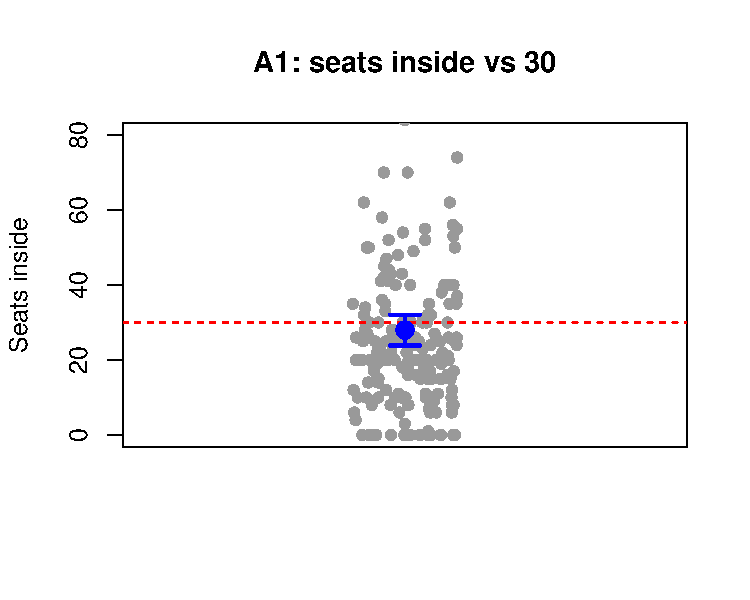
\includegraphics[width=.55\textwidth]{figures/A1_figure.pdf}
\caption{Seats inside each café (grey points), the mean with its 95\% CI (blue) and the benchmark of 30 seats (red dashed line). The y-axis is cut at 80 seats.}
\end{figure}
\begin{table}[H]\centering\caption{A1: one-sample t-test of the mean number of seats inside against 30.}\rtable{A1_table.tex}\end{table}

% ---------------------------------------------------------------------
\subsection{A2: Do cafés with outdoor seating have more seats inside?}
\Ho: the mean number of seats inside is the same in cafés with and without outdoor seating. \Hone: it is higher in cafés with outdoor seating (one-tailed, fixed in advance). Difference: outdoor minus no outdoor.
Method: Welch's t-test (the central limit theorem applies in both groups; Welch's test does not assume equal variances).
Cafés with outdoor seating have on average 30.6 seats inside, compared with 23.1 for cafés without, a difference of 7.5 seats (\CI{-0.4}{15.4}; \ncol\,=\,128 and 63, 4 cafés lost). Welch's one-tailed t-test finds evidence that cafés with a terrace are larger inside (\tstat{161.59}{1.87}, \pval{.031}), but the two-sided interval includes zero, so the evidence is modest. The effect is small (\textit{d}\,=\,0.26): about two extra tables.

\begin{figure}[H]\centering
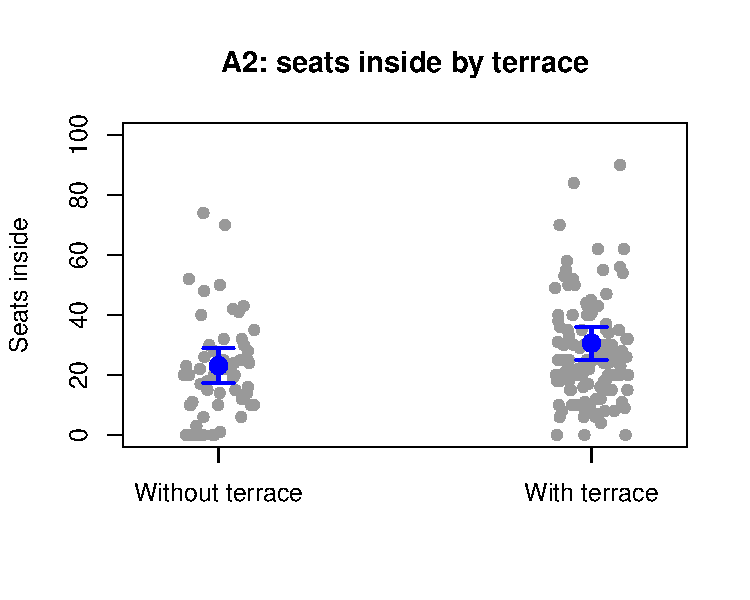
\includegraphics[width=.6\textwidth]{figures/A2_figure.pdf}
\caption{Seats inside by outdoor seating. Grey points are cafés; blue shows each group's mean with its 95\% CI. The y-axis is cut at 100 seats.}
\end{figure}
\begin{table}[H]\centering\caption{A2: seats inside by outdoor seating, Welch's t-test (p one-tailed).}\rtable{A2_table.tex}\end{table}

% ---------------------------------------------------------------------
\subsection{A3: How many more seats does a café have inside than outside?}
\Ho: the mean difference (inside minus outside) is 0. \Hone: it is greater than 0 (one-tailed).
Method: paired t-test on the differences (the central limit theorem applies).
On average, a café has 28.1 seats inside and 10.8 outside, so 17.3 more seats inside than outside (\CI{13.5}{21.2}, \ncol\,=\,191, 4 cafés lost). A paired t-test gives strong evidence of this difference (\tstat{190}{8.85}, \plt{.001}, one-tailed), and the effect is medium-sized (\textit{d}$_z$\,=\,0.64). Outdoor seating is an addition to a café rather than its main space, which matters in winter, when most terraces close.

\begin{figure}[H]\centering
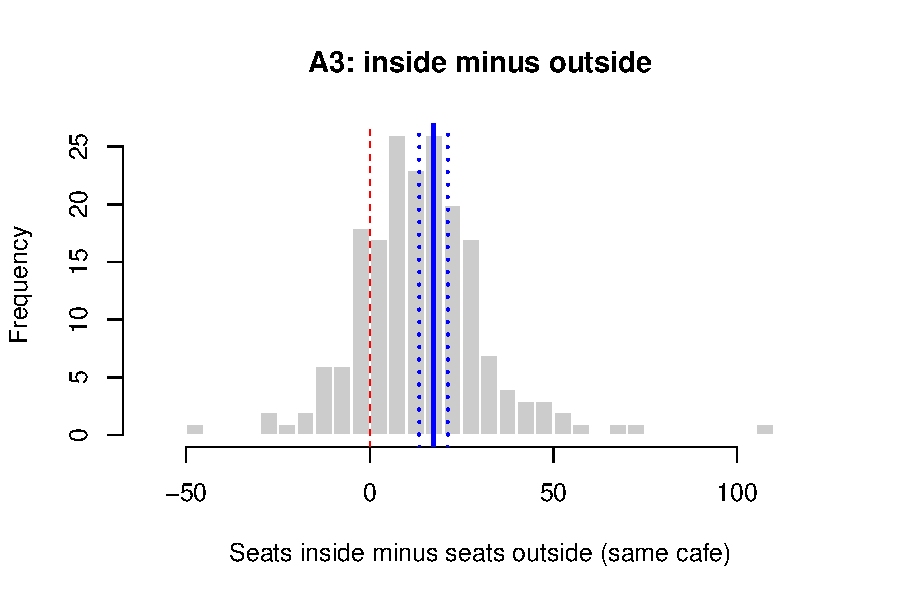
\includegraphics[width=.75\textwidth]{figures/A3_figure.pdf}
\caption{Distribution of the paired difference seats inside minus seats outside, with the mean difference (solid blue line), its 95\% CI (dotted blue lines) and zero difference (red dashed line). The x-axis is cut at $-60$ and 120.}
\end{figure}
\begin{table}[H]\centering\caption{A3: paired t-test of seats inside against seats outside (p one-tailed).}\rtable{A3_table.tex}\end{table}

% ---------------------------------------------------------------------
\subsection{A4: Does the number of outdoor seats differ between districts?}
\Ho: outdoor seats are distributed the same way in Prague 1, 2, 3, 5, 7 and 8. \Hone: at least one district differs.
Method: Kruskal--Wallis test with Dunn's pairwise comparisons (Holm adjustment), because Prague~2, 3 and 5 have fewer than 30 cafés and skewed counts (Table~\ref{tab:D}).
The mean number of outdoor seats ranges from 2.8 in Prague~5 to 14.0 in Prague~1 (\ncol\,=\,181; 14 cafés lie in other districts or have missing values). The Kruskal--Wallis test finds evidence that the districts differ (\textit{H}(5)\,=\,13.00, \pval{.023}). After Holm's adjustment for the 15 pairwise comparisons, only Prague~5 and Prague~1 differ (adjusted \pval{.008}; Table~\ref{tab:A4post}): cafés in Prague~5 have about 11 fewer outdoor seats on average, and more than half of them have none at all (median 0). Prague~5 against Prague~7 and Prague~8 comes close (adjusted \pval{.067} and \pval{.100}). Prague~5 has only 20 cafés, so this result rests on few observations.

\begin{figure}[H]\centering
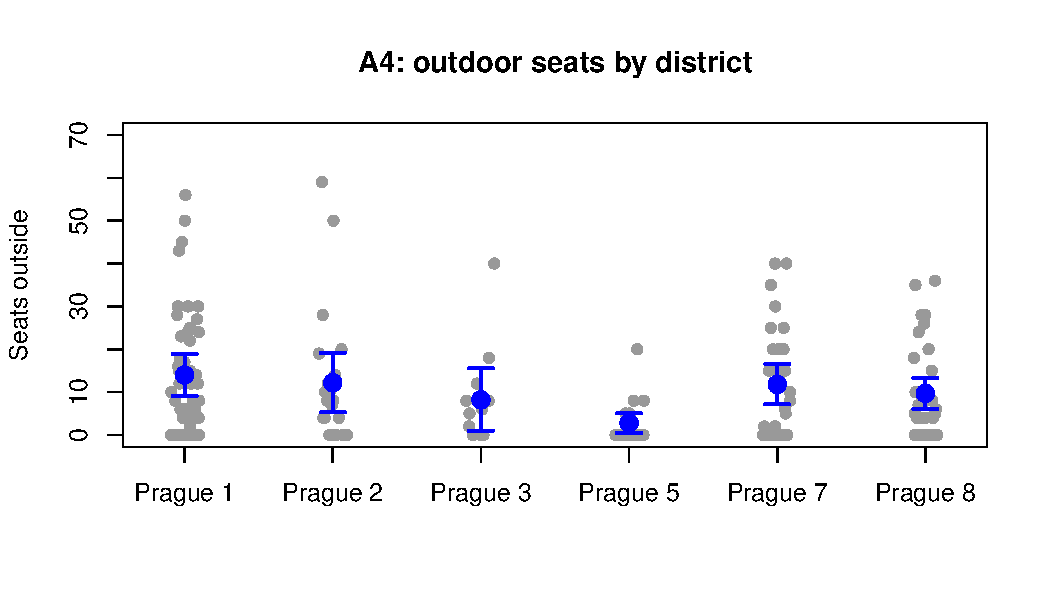
\includegraphics[width=.75\textwidth]{figures/A4_figure.pdf}
\caption{Outdoor seats per café in six districts (grey points), with each district's mean and 95\% CI (blue). The y-axis is cut at 70 seats.}
\end{figure}
\begin{table}[H]\centering\caption{A4: outdoor seats by district, with the Kruskal--Wallis test.}\rtable{A4_table.tex}\end{table}

% ---------------------------------------------------------------------
\subsection{A5: Are small cafés more likely to be top-rated?}
\Ho: the share of top-rated cafés (rating $\ge$ 4.7) is the same for small cafés ($\le$ 15 seats inside) and other cafés. \Hone: it is higher for small cafés (one-tailed). Difference: small minus other, in percentage points.
Method: $\chi^2$ test of independence; the smallest expected count is 20, so Fisher's exact test is not needed.
Of the small cafés, 58.5\% are top-rated, compared with 29.7\% of the other cafés: a difference of 28.8 percentage points (\CI{13.5}{44.1}, \Ncol\,=\,191). The test gives strong evidence of an association (\chisqstat{1}{191}{13.51}, \plt{.001}, one-tailed), with a small-to-medium effect (Cramér's \textit{V}\,=\,0.27). Small cafés are top-rated about twice as often, which is the strongest size effect in this report. It is an association, not a cause: for example, small cafés may have fewer, more loyal reviewers.

\begin{figure}[H]\centering
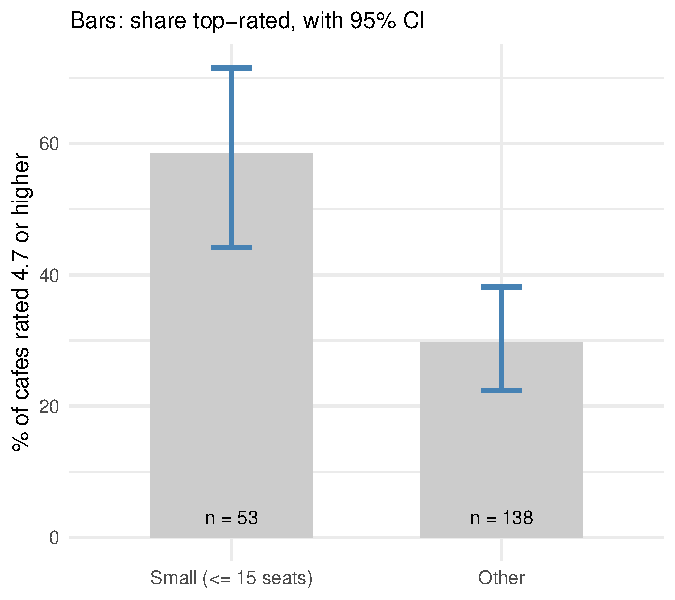
\includegraphics[width=.55\textwidth]{figures/A5_figure.pdf}
\caption{Share of top-rated cafés (Google rating 4.7 or higher) among small cafés and other cafés, with 95\% CIs.}
\end{figure}
\begin{table}[H]\centering\caption{A5: percentage of top-rated cafés by size, the difference in percentage points, the $\chi^2$ test (p one-tailed), Cramér's V and the smallest expected count.}\rtable{A5_table.tex}\end{table}

% ---------------------------------------------------------------------
\subsection{A6: Is the Price Level correlated with seats inside?}
\Ho: $\rho = 0$. \Hone: $\rho \neq 0$.
Method: Spearman's $\rho$ with a bootstrap CI. Seats inside is far from normal (skewness 4.4), and the central limit theorem concerns means, not the shape that Pearson's $r$ needs.
The correlation is positive but weak (Spearman's $\rho$\,=\,0.25, bootstrap \CI{0.09}{0.39}, \ncol\,=\,191, 4 cafés lost, \plt{.001}): larger cafés tend to be slightly more expensive, but size accounts for only about 6\% of the variation in prices.

\begin{figure}[H]\centering
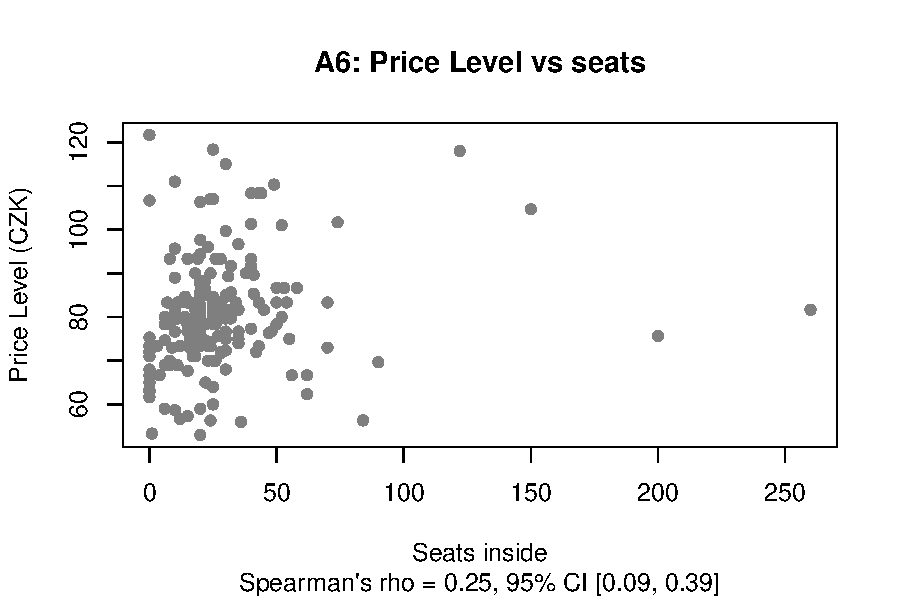
\includegraphics[width=.65\textwidth]{figures/A6_figure.pdf}
\caption{Price Level against seats inside; one point per café.}
\end{figure}
\begin{table}[H]\centering\caption{A6: Spearman correlation of Price Level and seats inside, with a bootstrap 95\% CI.}\rtable{A6_table.tex}\end{table}

% ---------------------------------------------------------------------
\subsection{A7: How much does the Price Level change per 10 seats?}
\Ho: slope $= 0$. \Hone: slope $\neq 0$.
Method: simple linear regression of the Price Level on seats inside (in units of 10 seats).
Each additional 10 seats inside go with a Price Level higher by 0.69\,CZK (\CI{0.07}{1.31}, \tstat{189}{2.19}, \pval{.030}, \ncol\,=\,191), and seats explain only 2\% of the variation in prices (\textit{R}$^2$\,=\,0.02). In practice this is tiny: a café with 50 more seats would be expected to charge about 3.5\,CZK more. The Breusch--Pagan test shows no problem with the spread of the residuals (\pval{.157}), but the slope depends strongly on a few very large cafés, above all VNITROBLOCK (260 seats, Cook's distance 0.54), Café Louvre (0.25) and Starbucks Reserve (0.20) (Appendix~\ref{app:diag}).

\begin{figure}[H]\centering
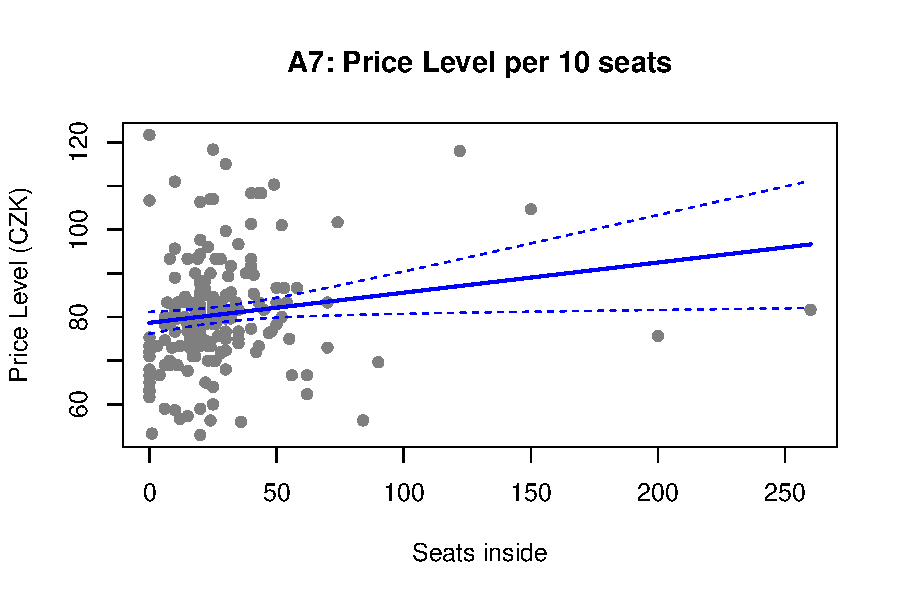
\includegraphics[width=.65\textwidth]{figures/A7_figure.pdf}
\caption{Price Level against seats inside, with the fitted regression line (solid) and its 95\% confidence band (dashed).}
\end{figure}
\begin{table}[H]\centering\caption{A7: simple regression of Price Level on seats inside (per 10 seats).}\rtable{A7_table.tex}\end{table}

% ---------------------------------------------------------------------
\subsection{A8: Does the link hold once distance from the Orloj is controlled?}
\Ho: the slope of seats inside, holding distance constant, is 0. \Hone: it is not 0.
Method: multiple regression of the Price Level on seats inside (per 10) and distance from the Orloj (km).
After adding the distance from the Orloj, the seats slope falls only slightly, from 0.69 to 0.61\,CZK per 10 seats (88\% remains), but it is no longer clearly different from zero (\CI{-0.01}{1.23}, \pval{.055}, \ncol\,=\,191, \textit{R}$^2$\,=\,0.05). Distance itself matters: each kilometre from the Orloj goes with a Price Level 1.55\,CZK lower (\CI{-2.91}{-0.19}, \pval{.025}). Location therefore explains little of the size--price link, but with both in the model the evidence for a size effect becomes weak. The Breusch--Pagan test gives \pval{.098}, so ordinary standard errors are kept.

\begin{figure}[H]\centering
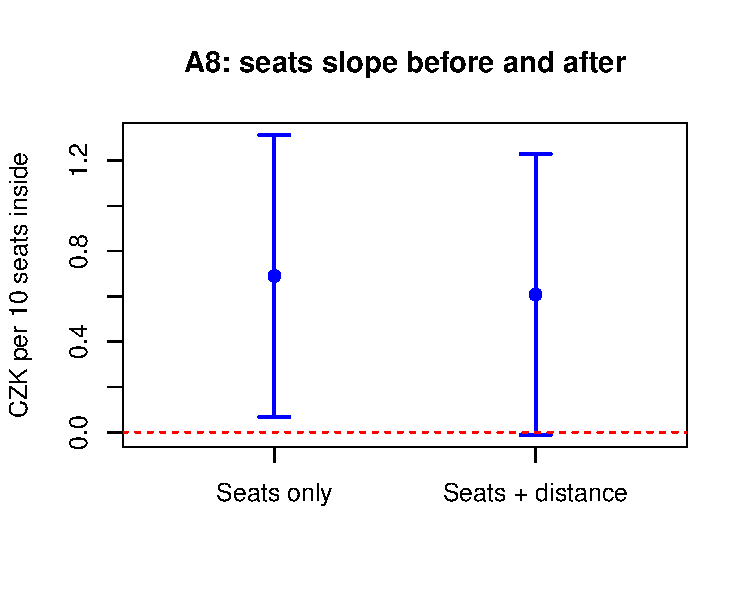
\includegraphics[width=.55\textwidth]{figures/A8_figure.pdf}
\caption{Slope of seats inside (CZK per 10 seats) with its 95\% CI, without and with distance from the Orloj in the model; the red dashed line marks no effect.}
\end{figure}
\begin{table}[H]\centering\caption{A8: multiple regression of Price Level on seats inside and distance from the Orloj, with the seats slope before distance was added.}\rtable{A8_table.tex}\end{table}

% ---------------------------------------------------------------------
\subsection{A9: Does the link differ with and without outdoor seating?}
\Ho: the interaction coefficient is 0 (same slope). \Hone: it is not 0.
Method: regression of the Price Level on seats inside, outdoor seating and their interaction.
For cafés without outdoor seating, each 10 seats go with a Price Level 2.75\,CZK higher (\CI{1.39}{4.10}). For cafés with outdoor seating, the slope is 2.62\,CZK lower (\CI{-4.15}{-1.10}, \tstat{185}{-3.41}, \plt{.001}), so it is essentially flat (about 0.13\,CZK per 10 seats; \ncol\,=\,189, \textit{R}$^2$\,=\,0.08; Breusch--Pagan \pval{.829}). Larger cafés are more expensive only when they have no terrace. This result should be read with care: the group without outdoor seating has only 62 cafés, and Café Slavia, a large and expensive café without a terrace, has a strong influence on it (Cook's distance 0.33).

\begin{figure}[H]\centering
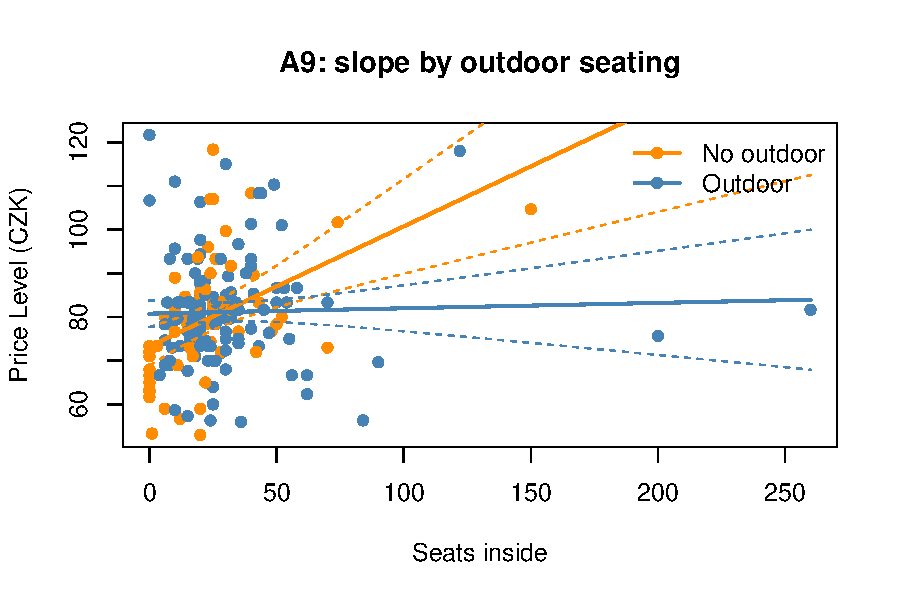
\includegraphics[width=.7\textwidth]{figures/A9_figure.pdf}
\caption{Price Level against seats inside, with separate regression lines and 95\% bands for cafés without (orange) and with (blue) outdoor seating.}
\end{figure}
\begin{table}[H]\centering\caption{A9: regression with the interaction of seats inside and outdoor seating.}\rtable{A9_table.tex}\end{table}

% ---------------------------------------------------------------------
\subsection{A10: Does the chance of an above-median Price Level change with size?}
\Ho: the average marginal effect of 10 seats is 0. \Hone: it is not 0.
Method: logistic regression of an above-median Price Level on seats inside (per 10), reported as the average marginal effect.
Each additional 10 seats inside raise the predicted probability of an above-median Price Level by 2.7 percentage points on average (\CI{-0.3}{5.7}, \textit{z}\,=\,1.77, \pval{.077}, \ncol\,=\,191; odds ratio 1.12). There is no evidence that the chance of being among the more expensive half of cafés depends on size. The direction agrees with A6 and A7, but the effect is small and uncertain.

\begin{figure}[H]\centering
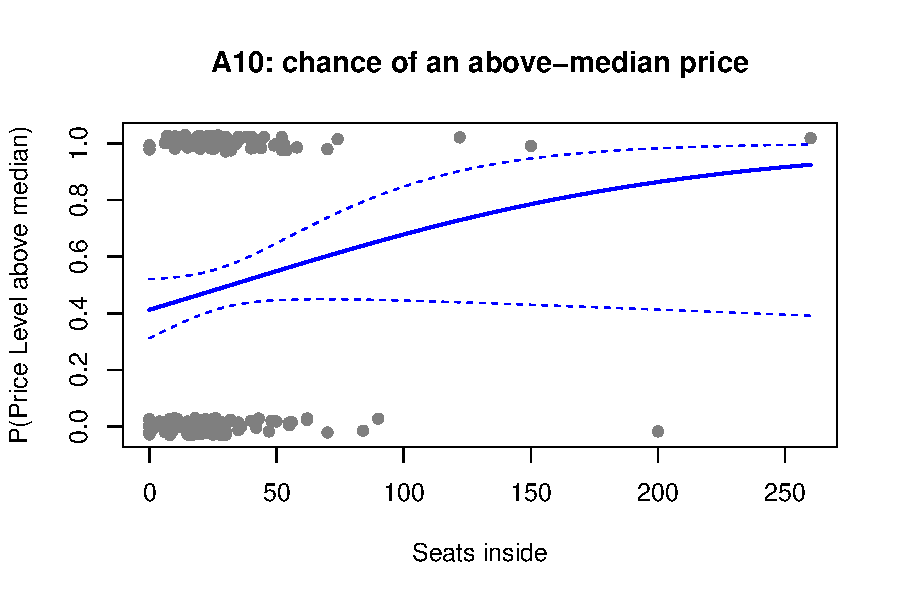
\includegraphics[width=.65\textwidth]{figures/A10_figure.pdf}
\caption{Cafés with an above-median (1) or not (0) Price Level against seats inside, with the predicted probability from the logistic regression (solid) and its 95\% CI (dashed).}
\end{figure}
\begin{table}[H]\centering\caption{A10: logistic regression of above-median Price Level on seats inside: average marginal effect in percentage points and odds ratio.}\rtable{A10_table.tex}\end{table}

% =====================================================================
\section{Discussion and limitations}
Taken together, the results describe a market of mostly small cafés. Half have 22 seats or fewer, the typical café has about 17 more seats inside than outside, and outdoor seating is most common in Prague~1 and least common in Prague~5. Size is clearly linked to ratings: small cafés are top-rated about twice as often as larger ones. The link between size and price is much weaker. Bigger cafés are slightly more expensive (A6, A7), but by less than one crown per 10 seats. The link is no longer clearly different from zero once distance from the Orloj is controlled (A8) or when price is treated as above or below the median (A10). It appears only among cafés without outdoor seating (A9), where a few large historic cafés drive it.

The results have three main limits. First, the sample is a convenience sample: students chose which cafés to visit, mostly in the centre, so every result holds \emph{in this sample} and not necessarily for all Prague cafés. Second, the data are observational, so none of the associations is causal; for example, small cafés may be better rated because they have fewer, more loyal reviewers and not because being small makes them better. Third, cafés in the same district share rents, tourist flows and competition, so they are not independent observations. Every test here assumes independence, so the standard errors are probably too small and the p-values too optimistic. In addition, seat counts were partly estimated by students, some prices were taken as the first of several listed sizes, and the regressions depend on a handful of very large cafés.

\section{Conclusion}
How big are Prague's cafés, and does size matter? In this sample, the typical café is small, with about 22 seats inside and a modest terrace. Size goes clearly with ratings, because small cafés are much more often top-rated, but only weakly with prices: bigger cafés charge at most about one crown more per 10 seats, and this link disappears once location is taken into account. Size tells us more about how a café is rated than about what it charges.

% =====================================================================
\appendix
\section{Descriptive statistics}\label{app:desc}
\begin{table}[H]\centering\caption{Descriptive statistics of every variable and group used: n, mean, standard deviation, median, interquartile range, minimum and maximum.}\rtable{D_stats.tex}\end{table}
\begin{table}[H]\centering\caption{Yes/no variables: counts and the percentage of yes.}\rtable{D_categorical.tex}\end{table}

\section{Normality and central-limit checks}
Each row: histogram, boxplot, normal Q--Q plot and the distribution of 5{,}000 bootstrapped means (seed 2026).
\begin{figure}[H]\centering
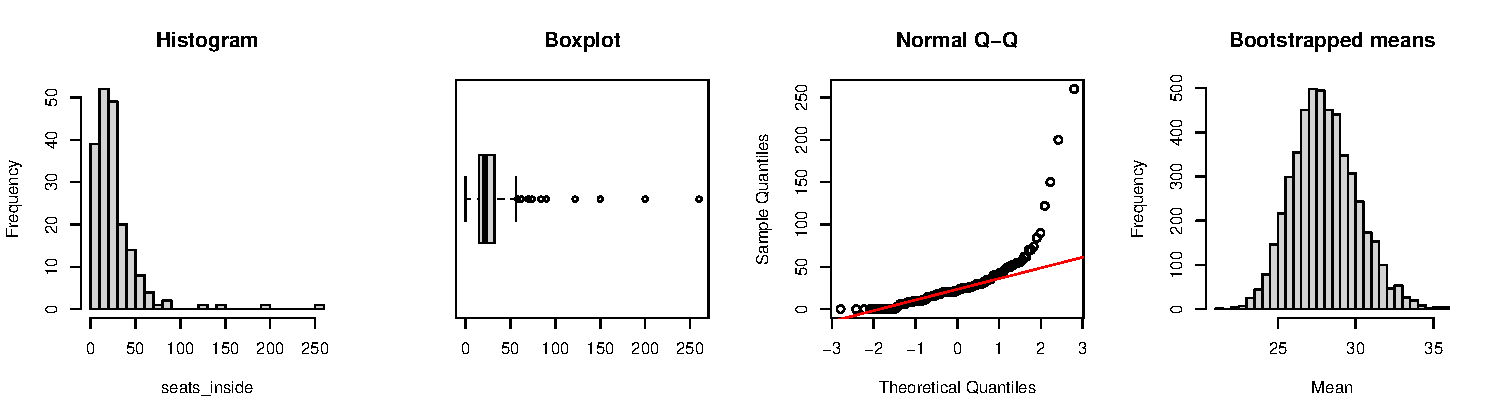
\includegraphics[width=\textwidth]{figures/D_seats_inside.pdf}\\
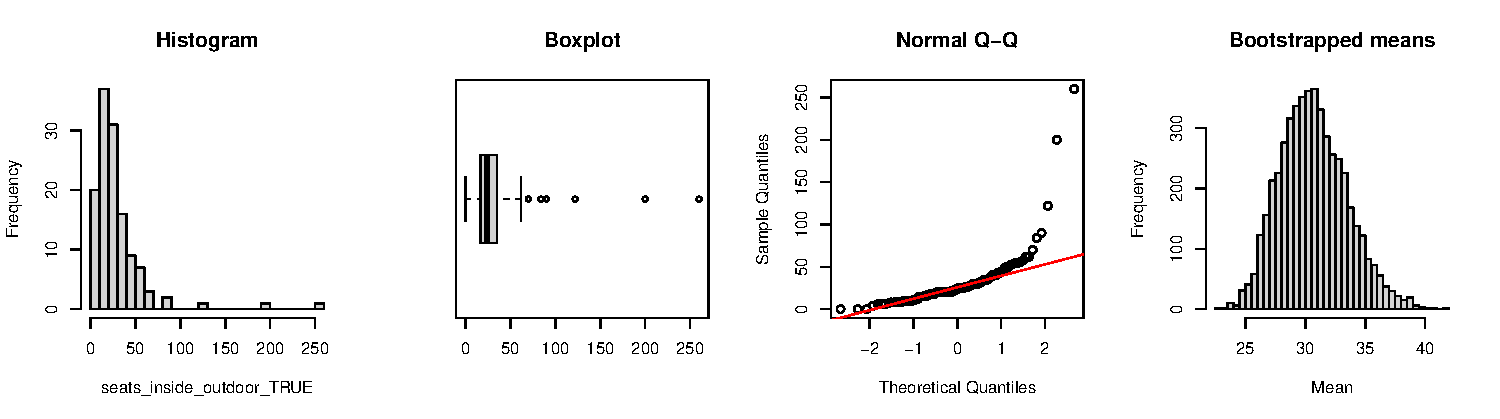
\includegraphics[width=\textwidth]{figures/D_seats_inside_outdoor_TRUE.pdf}\\
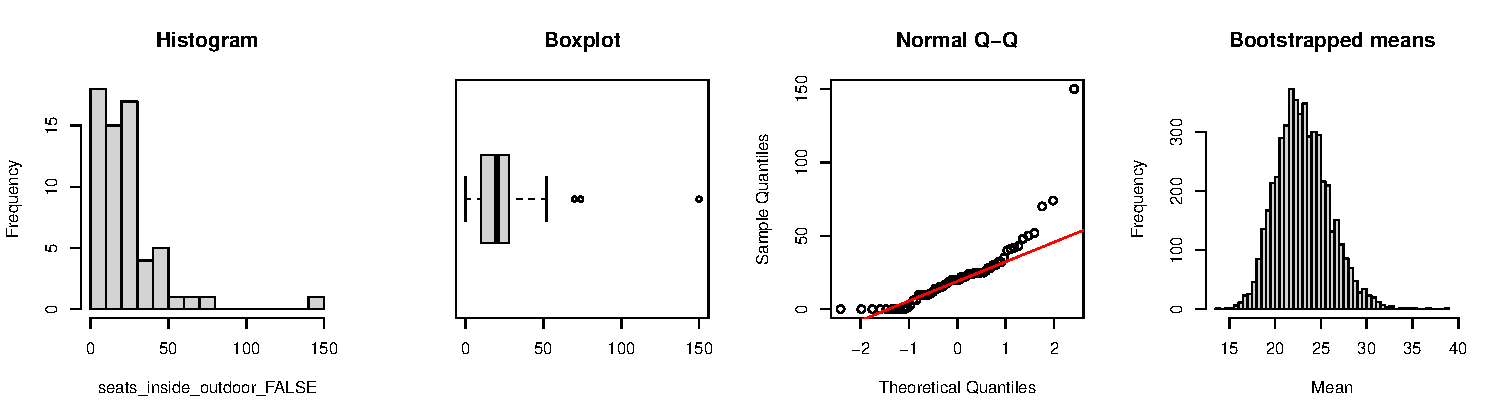
\includegraphics[width=\textwidth]{figures/D_seats_inside_outdoor_FALSE.pdf}\\
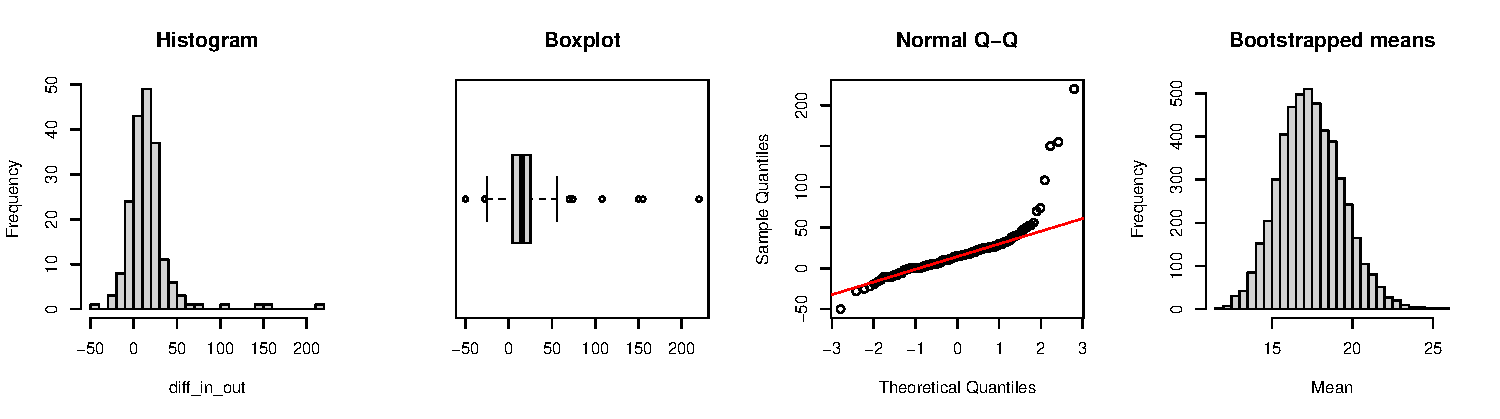
\includegraphics[width=\textwidth]{figures/D_diff_in_out.pdf}
\caption{Seats inside (all cafés; with and without outdoor seating) and the paired difference inside minus outside.}
\end{figure}
\begin{figure}[H]\centering
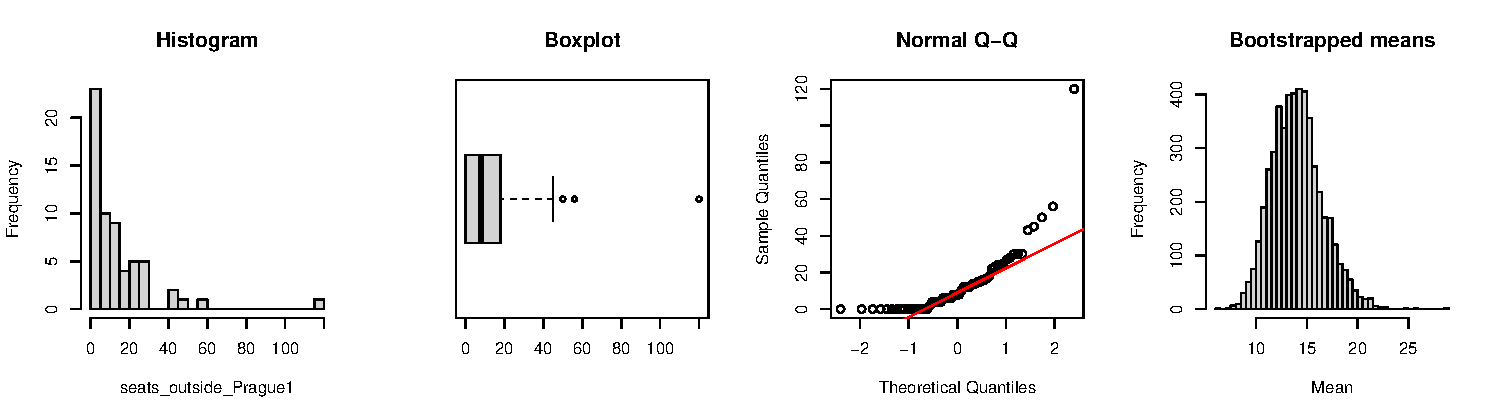
\includegraphics[width=\textwidth]{figures/D_seats_outside_Prague1.pdf}\\
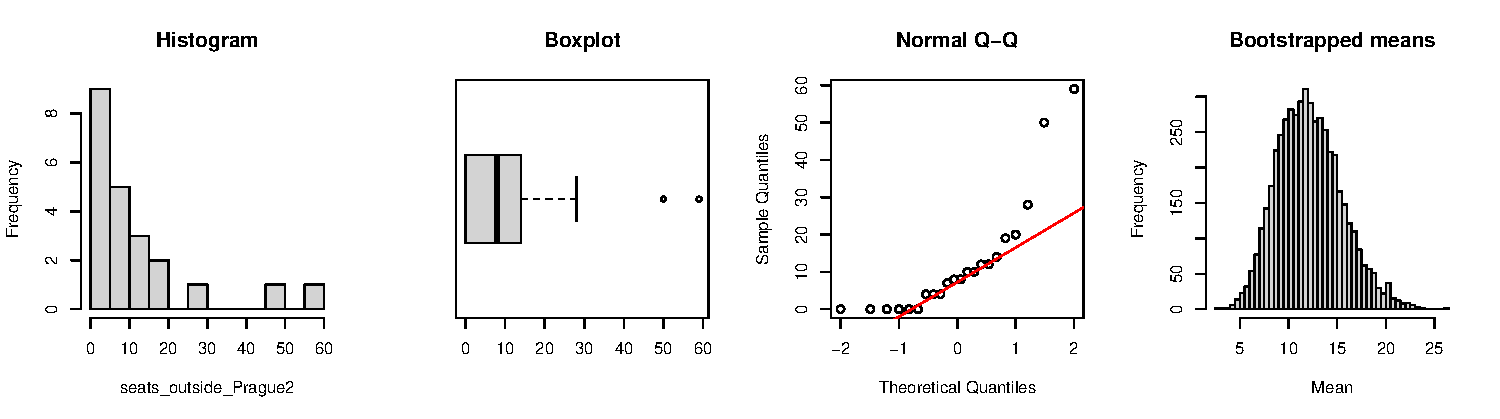
\includegraphics[width=\textwidth]{figures/D_seats_outside_Prague2.pdf}\\
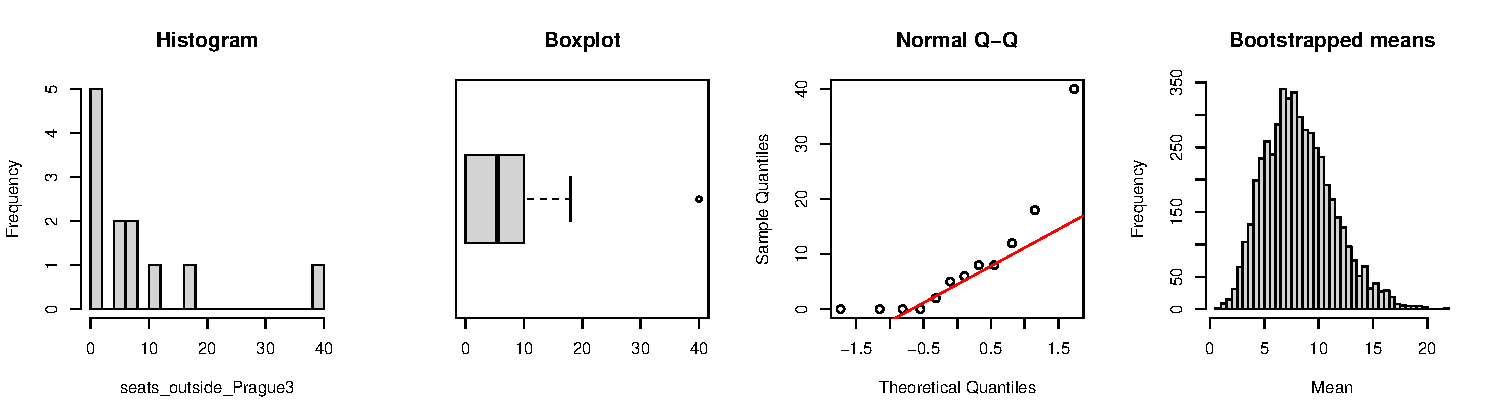
\includegraphics[width=\textwidth]{figures/D_seats_outside_Prague3.pdf}
\caption{Seats outside in Prague 1, 2 and 3.}
\end{figure}
\begin{figure}[H]\centering
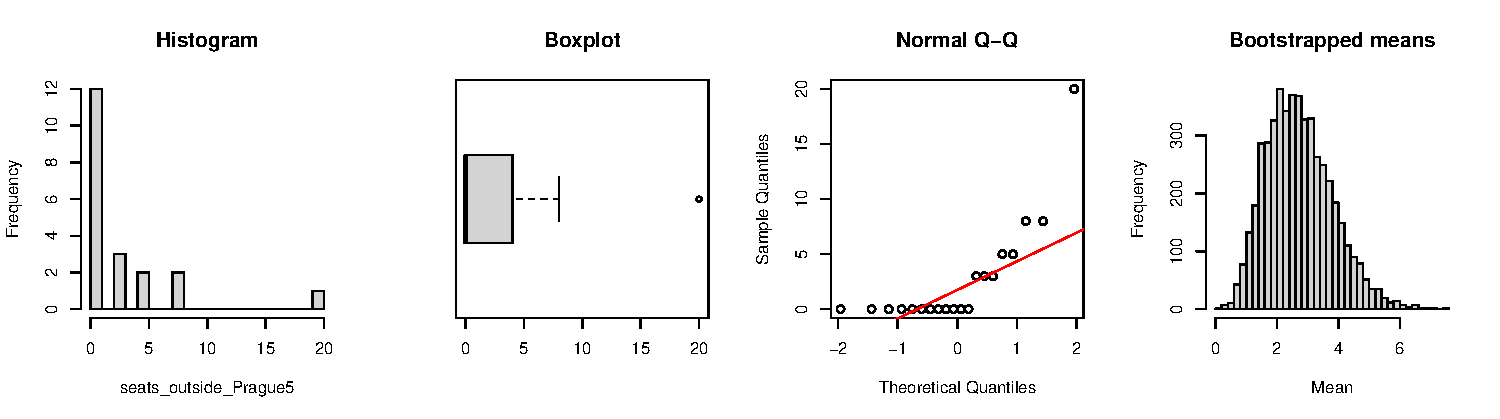
\includegraphics[width=\textwidth]{figures/D_seats_outside_Prague5.pdf}\\
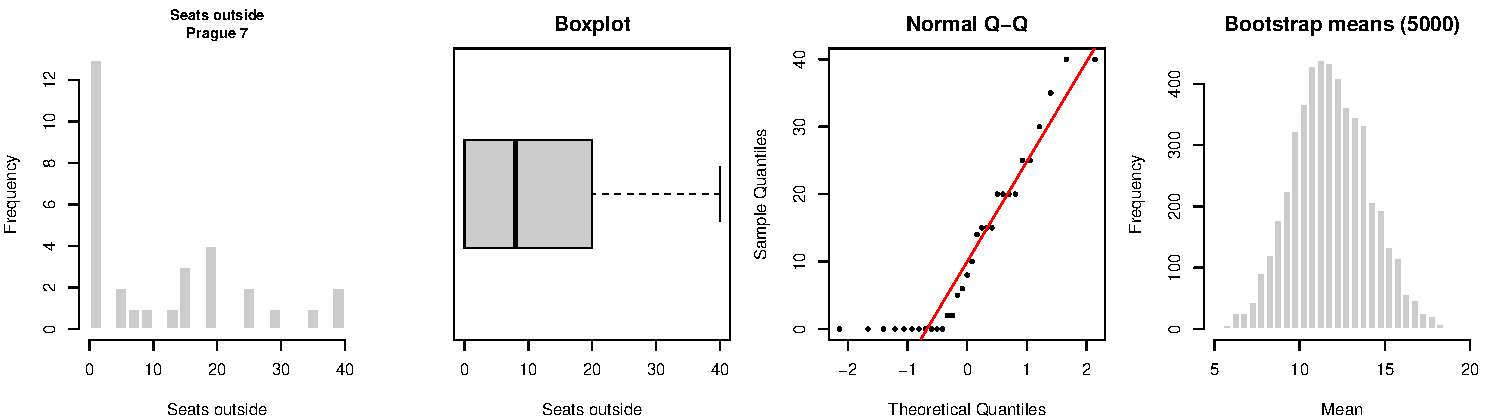
\includegraphics[width=\textwidth]{figures/D_seats_outside_Prague7.pdf}\\
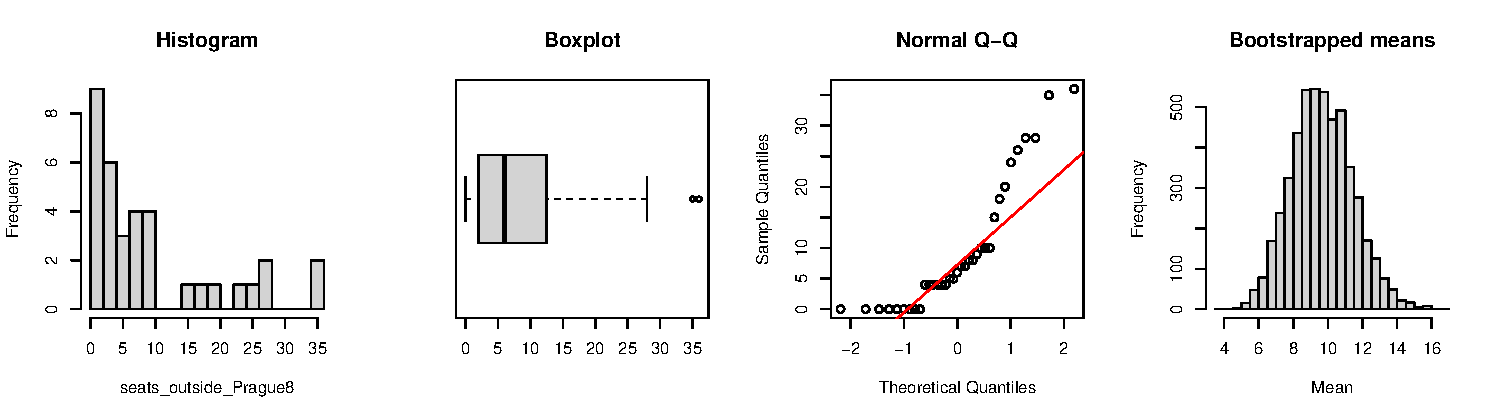
\includegraphics[width=\textwidth]{figures/D_seats_outside_Prague8.pdf}
\caption{Seats outside in Prague 5, 7 and 8.}
\end{figure}
\begin{figure}[H]\centering
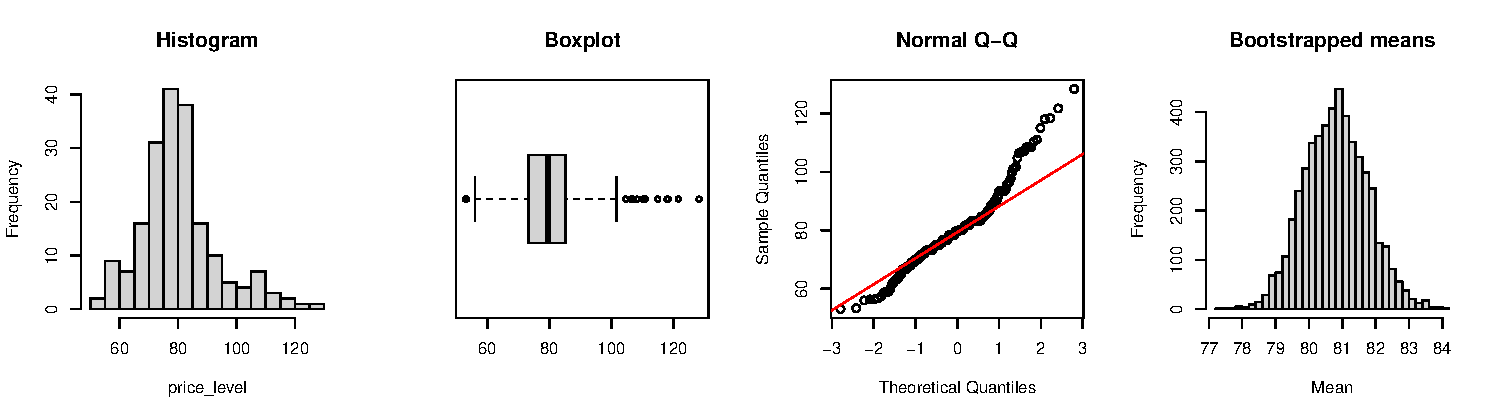
\includegraphics[width=\textwidth]{figures/D_price_level.pdf}\\
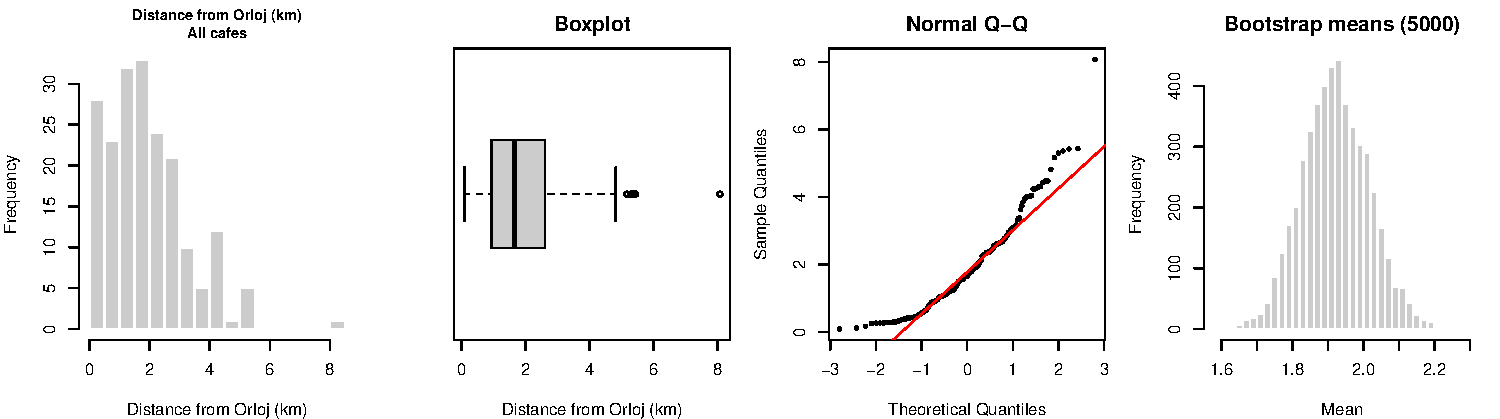
\includegraphics[width=\textwidth]{figures/D_dist_orloj.pdf}
\caption{Price Level and distance from the Orloj.}
\end{figure}

\section{Assumption checks and post hoc tests}\label{app:diag}
\begin{table}[H]\centering\caption{A4: Dunn's pairwise comparisons: z statistics, raw and Holm-adjusted p-values.}\label{tab:A4post}\rtable{A4_posthoc_table.tex}\end{table}
\begin{figure}[H]\centering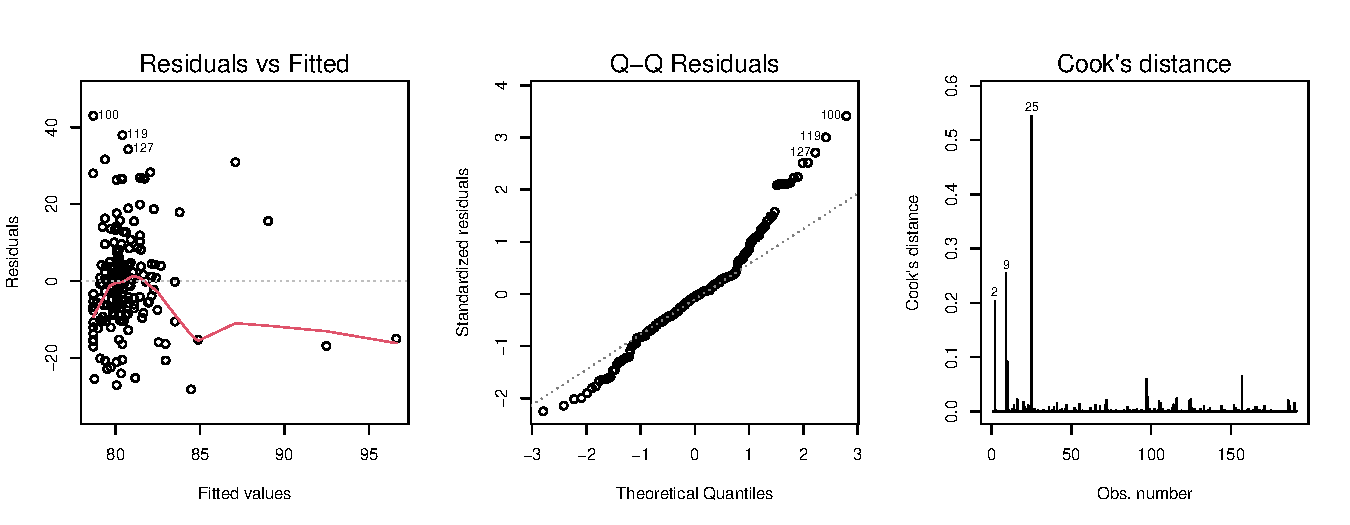
\includegraphics[width=\textwidth]{figures/A7_diagnostics.pdf}\caption{A7 diagnostics: residuals vs fitted, normal Q--Q of residuals, Cook's distance.}\end{figure}
\begin{figure}[H]\centering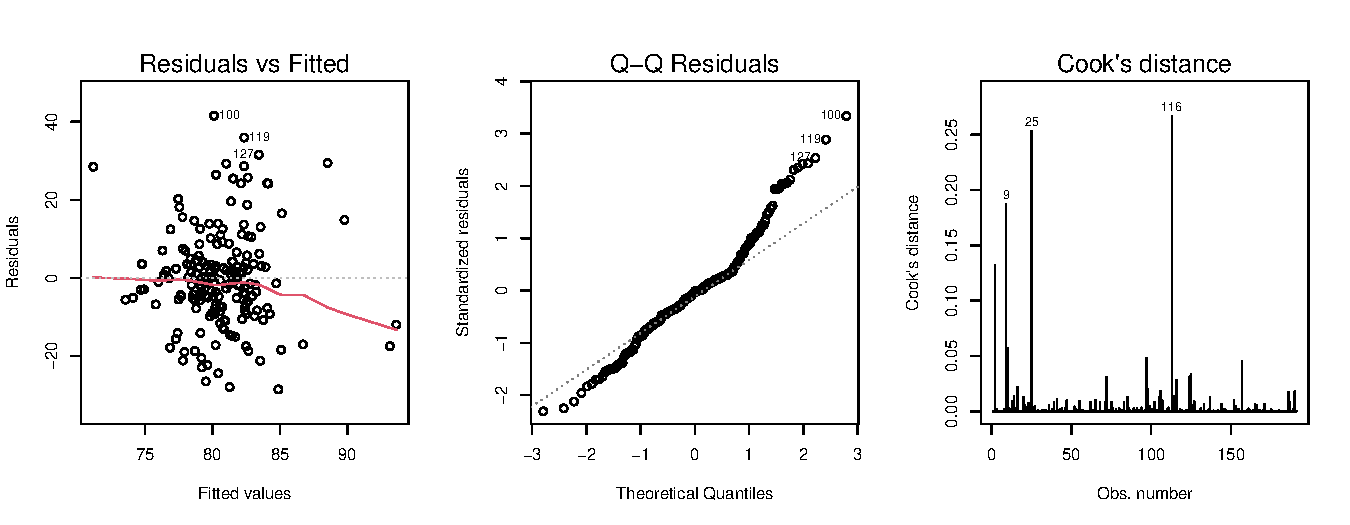
\includegraphics[width=\textwidth]{figures/A8_diagnostics.pdf}\caption{A8 diagnostics: residuals vs fitted, normal Q--Q of residuals, Cook's distance.}\end{figure}
\begin{figure}[H]\centering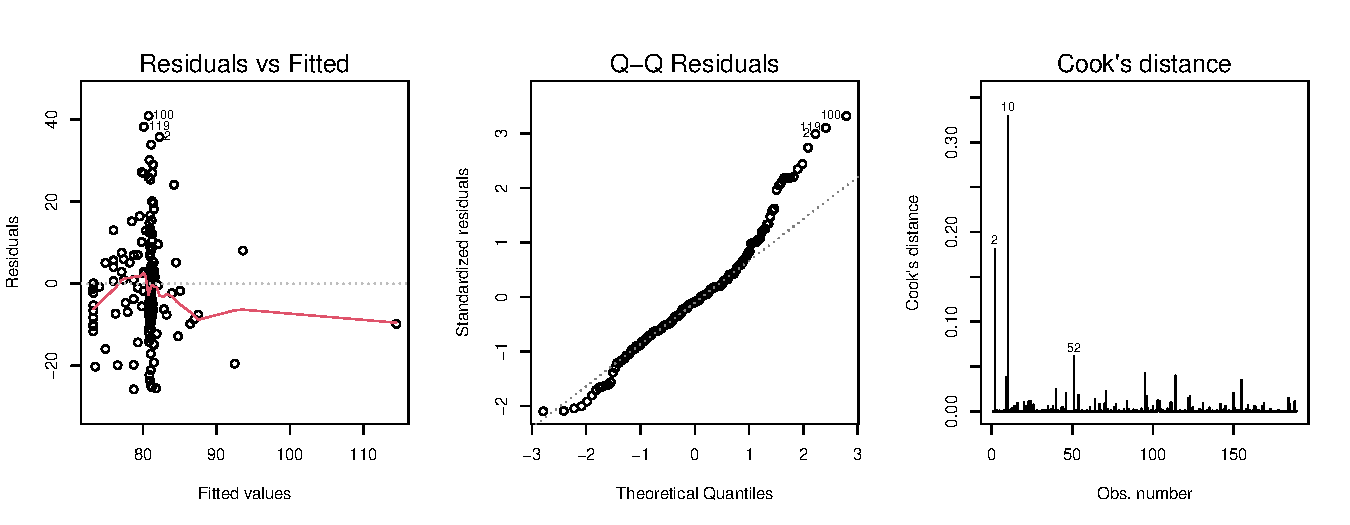
\includegraphics[width=\textwidth]{figures/A9_diagnostics.pdf}\caption{A9 diagnostics: residuals vs fitted, normal Q--Q of residuals, Cook's distance.}\end{figure}
The Breusch--Pagan test does not reject constant residual variance in any regression (A7 \pval{.157}, A8 \pval{.098}, A9 \pval{.829}), so ordinary standard errors are reported. The residuals are right-skewed in the Q--Q plots, but with 189--191 cafés the coefficients are still approximately normal. Using the threshold $4/n \approx 0.021$, several cafés are influential; the largest Cook's distances are VNITROBLOCK (0.54 in A7, 0.25 in A8), Café Louvre (0.25 in A7), Kavárna Creperié (0.27 in A8), Starbucks Reserve (0.20 in A7, 0.18 in A9) and Café Slavia (0.33 in A9). These very large or very expensive cafés matter for the size--price slopes, as discussed in the results. They are real cafés and not data errors, so they were kept.

\end{document}
